% !TEX root = ../00_thesis.tex

% ------------------------------------------------------------------------------
\section{Performance of the \TTW Scheduler}
\label{sec:ttw_evaluation_sched}
% ------------------------------------------------------------------------------

The following two sections present the performance evaluation of our \TTW implementation, presented in~\cref{sec:ttw_implementation}.
We first evaluate the performance of the scheduler. In particular, we illustrate the benefits of the minimal inheritance strategy presented in \cref{sec:multi_mode} and we show that the complexity of the schedule synthesis is tractable.

% ------------------------------------------------------------------------------
\subsection{Benefits of Minimal Inheritance}

\begin{figure}
  \centering
  \href{\ttwfig{Figure-11}}{%
  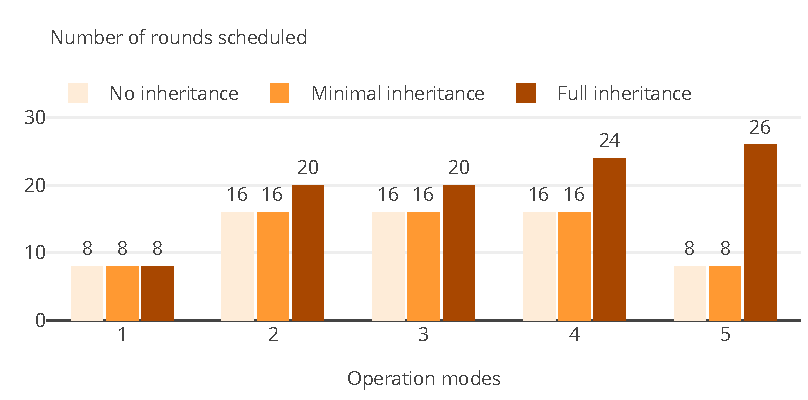
\includegraphics[scale=1]{inheritance_eval}}
  \caption{Number of rounds in the different modes' schedule, depending on the inheritance approach considered.
  \capt{We consider the number of rounds scheduled over 80\s, which is the least common multiple of the modes' hyperperiod.}}
  \label{fig:inheritance_eval}
\end{figure}

Every round introduces some overhead (mainly from  sending the beacon), which consumes energy.
To reduce the energy consumption, \TTW aims to minimize the number of rounds \objective{1}.
The schedule synthesis for a single mode is optimal in this respect; that is, the procedure guarantees that the schedule minimizes the number of communication rounds~(\cref{sec:single_mode}).

The second objective of the scheduler is to allow persistent applications to keep the same schedule in different operation modes \objective{2}.
This creates additional constraints that break the optimality guarantee: in other words, the schedule of mode \modej, when constrained to be compatible with mode \modei, may contain more rounds that required to schedule the mode \modej alone.
A naive solution to meet \objective{2} is to completely ``reserve the space'' of previously scheduled modes. This is equivalent to consider that all applications executing in mode \modei are also executing in \modej, even if it is not actually the case. We call this the \emph{full inheritance} approach.
This approach does guarantee compatibility but it is very pessimistic: it leads to an excessive increase of the number of rounds and find problems to be non-schedulable when they may in fact be feasible.


\begin{figure}
  \centering
  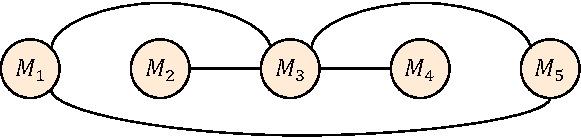
\includegraphics[scale=1]{modeGraph_eval}
  \caption{The mode graph \modeGraph' used in the inheritance evaluation scenario.
  Mode \modei has priority $i$. The applications executing in each mode are listed in~\cref{append:inheritance_eval}.}
  \label{fig:modeGraph_eval}
\end{figure}


In \cref{sec:multi_mode}, we derived the minimal set of constraints that are necessary to guarantee the compatibility between modes \objective{2}, which we refer to as \emph{minimal inheritance}.
We now illustrate with a simple example that the minimal inheritance does not overly increase the number of communication round required and performs much better than the full inheritance.
%
We consider the following configuration (fully detailed in \cref{append:inheritance_eval}): The system is composed of 13 nodes, running 15 different applications including 45 tasks and 30 messages.
The periods and deadlines vary between 10 and 80\s. The applications are executing in 5 different modes connected by the mode graph shown in~\cref{fig:modeGraph_eval}.
Finally, all applications are considered persistent.
We synthesize the schedule for the 5 modes while considering
(i)~no inheritance,%
%
\footnote{Considering no inheritance is equivalent to set all applications as non-persistent. In other words, there are no constraints between the different modes and the individual mode schedules are guaranteed to be optimal in terms of number of rounds~(\cref{sec:single_mode}).}
%
(ii)~our minimal inheritance approach, and (iii)~the naive full inheritance approach.
The results are shown in \cref{fig:inheritance_eval}.

One important observation is that the number of rounds steadily increases with the full inheritance approach, which is expected: the full inheritance assumes that all previously scheduled applications are still executing. Thus, the number of applications to schedule only increases, and so does the number of round required. Ultimately, this not only wastes energy, it also limits scalability with the number of operation modes.
In comparison, our minimal inheritance approach performs much better: Since only the required constraints are included, the minimal inheritance does not suffer from the scalability issue mentioned above. In this example, the minimal inheritance performs optimally (\ie it does not schedule more rounds that the minimum, captured by the ``no inheritance'' case); but note that this is {\bf not true in general}, it simply happens to be the case in this example.

\fakepar{Conclusion}
The minimal inheritance approach derived in \cref{sec:multi_mode} efficiently addresses the challenge of synthesizing compatible schedules~\objective{2} while minimizing the energy impact in terms of number of rounds scheduled~\objective{1}.
This approach does increase the complexity of the synthesis formulation; however, it is implemented in our \TTW scheduler, it induces no overhead for the user, and it does not affect the synthesis solving time, as discussed below.

% ------------------------------------------------------------------------------
\subsection{Offline Solving Time}

We computational complexity of the schedule synthesis is made tractable by \TTW's sequential approach: modes are scheduled individually, in order of priority~(\cref{sec:multi_mode}) and for each mode, the number of rounds to schedule is kept fixed then incremented until a solution is found~(\cref{sec:single_mode}).

For the evaluation scenario described above, the solving time for one mode grows up to ten minutes~(\cref{table:solvingTimes}) and is generally correlated with the complexity of the mode to schedule: mode \mode{3} and \mode{4} contains the most applications~(\cref{append:inheritance_eval}), leading to more constraints in the formulation.
Furthermore, we note that the minimal inheritance strategy does not increase the overall solving time compared to ``no inheritance''. The intuition is that, by reserving some applications' schedule, we fix the value of some of the problem variables, thereby reducing the complexity of the problem.
However, as shown by the full inheritance approach, if too many variables are fixed, the resulting problem might become harder to solve: more communication rounds become required, which increases the number of variables and thus the complexity.

\fakepar{Conclusion}
The evaluation scenario is simple but representative of a middle-sized \CPS. Our evaluation shows that the computational complexity may grow to the scale of minutes for challenging modes, which remains perfectly tractable for a task that needs to be performed only once and before deployment.

\begin{table}
  \centering
  \caption{Approximate solving time for the different modes of the inheritance evaluation~(\cref{sec:ttw_evaluation_sched}).
  \capt{Time expressed in seconds; all computation performed on a commodity laptop.}}
  \label{table:solvingTimes}
  {\smaller \input{\TablePath/solvingTimes.csv}}
\end{table}






% -----------------------------------------------------------------------------
\section{Performance of \TTnet}
\label{sec:ttw_evaluation_implem}
% ------------------------------------------------------------------------------

After the evaluation of the \TTW scheduler~(\cref{sec:ttw_evaluation_sched}), we now consider the performance of our \TTnet implementation, described in \cref{subsec:implem_ttnet}.

% ------------------------------------------------------------------------------
\subsection{Memory Utilization}

First, we consider the memory utilization induced by storing the scheduling tables in the nodes' memory.
For a given operation mode, the entire schedule contains the task offsets, the message offsets and deadlines, the round starting times, and the allocations of messages to rounds~(\cref{table:ttw_inputs_outputs}).
In addition, nodes must know the task periods and the mode hyperperiod to compute the absolute start time of the tasks and rounds.

Since we dedicate the execution of tasks and the wireless communication to different processors~(\cref{sec:ttw_implementation}), the memory cost for storing the schedule can be splitted.
On the application side, we must store the task offsets and periods, which are required to know when to execute the tasks; \ie 2 variables per task.
On the communication side, we must store the mode hyperperiod and the rounds information, \ie the offset and allocation of the rounds scheduled within the mode's hyperperiod; \ie $(\nslotsmax+1)$ variables per round.
The message deadlines are not required at runtime and do not need being stored.
As a result, we can generally estimate that the scheduling tables represent tens to hundreds of variables per mode for each processor.

\fakepar{Conclusion}
Our application and communication processors feature 64\kB~\cite{msp432} and 4\kB\cite{CC430F6137} of RAM, respectively. Thus, considering an average size of two\bytes per variable, storing the scheduling tables represent a significant overhead and limits the scalability of the system, in particular on the communication processor.
This limitation would be significantly relaxed with newer platforms, which commonly feature 256\kB of RAM~\cite{nRF52840}.

% ------------------------------------------------------------------------------
\subsection{\TTnet Model}
\label{subsec:model}
As discussed in \cref{sec:ttw_implementation}, we implement \TTnet using \baloo, which allows to derive a precise model of
(i)~the execution time of a communication round and
(ii)~the time spent with the radio turned on, which correlates with the energy consumed for communication.
Estimating the communication time is necessary to synthesize the schedules since the scheduler must know how long the rounds last.
This model should be as tight as possible not to ``waste'' time and thus minimize the end-to-end deadlines schedulable by \TTW, but it must be a safe upper-bound in order to prevent deadline misses.
This section presents our \TTnet model and derives the theoretically achievable performance in terms of minimal message latency and the energy savings expected from using rounds.

Let $\app.\delta$ denote the latency of an application \app. This latency represents the delay for a complete execution of \app; that is, the completion of all tasks in \app.\predG. Let $\app.c$ be a \emph{chain} in \app.\predG.
A chain is defined as a path of \app.\predG starting with a task without predecessor and ending with a task without successor.%
%
\footnote{For example, $(\tau_2, m_2, \tau_4)$ is a chain of \predG in \cref{fig:precedence_graph}.}
%
The minimum achievable latency for a single message in \TTW is the length of a round composed of only one slot, denoted $\Tround(L,1)$ where $L$ is the payload size. Thus $\app.\delta$ is lower-bounded by
\begin{align}
\label{eq:min_deadline}
\app.\delta \;
	& \geq \; \max_{\app.c \,\in\, \app.\predG}
		\left(
			\; \sum_{\tau \, \in \, \app.c} \tau.e \,+\, \sum_{m \, \in \, \app.c} \Tround(L,1) \;
		\right)
\end{align}

\begin{remark}
  By comparison, the best possible guarantee for the latency of a single message provided by  \DRP~(\cref{ch:drp}) is of the order of $2*\Tround(L,\nslotsmax)$.
  Since $\Tround(L,\nslotsmax) \approx \nslotsmax*\Tround(L,1)$, \TTW reduces the minimal guarantee on message latency by a factor of approximately $2*\nslotsmax$.
  For a relatively small number of slots per round, such as $\nslotsmax=5$, this represents an order of magnitude improvement.
  This difference stems from the loose coupling between the task and message schedules in \DRP, whereas \TTW statically schedules all tasks and messages.
\end{remark}


\afterpage{
\begin{figure}
\centering
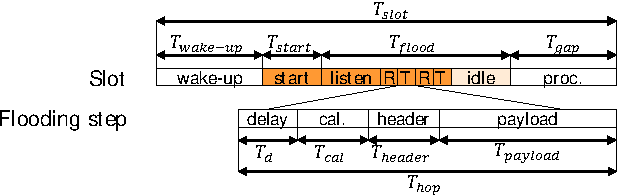
\includegraphics[scale=1]{Tslot}
\caption{%
Break-down of a communication round.
\capt{%
At the slot level, the colored boxes identify phases where the radio is on.
In the ``idle'' phase, the radio is turned off in practice, but this idle time depends on each node's distance to the initiator.
To estimate the energy saving of rounds (\cref{fig:energy_ratio}), we assume that the radio stays on for the whole time of \Tglossy, as specified in~\cref{eq:Ton}.
}
}
\label{fig:Tslot}
\end{figure}}

A round \Tround is composed of up to $(\nslotsmax+1)$ slots in which Glossy floods~\cite{ferrari2011Glossy} are executed.
An entire slot completes in time $\Tslot$, decomposed into
\begin{equation}
  \Tslot = \Twakeup + \Tstart + \Tglossy + \Tgap
\end{equation}
The composition of a slot in our implementation is detailed in~\cref{fig:Tslot}.
First, all nodes wake up (\Twakeup) and switch on their radio (\Tstart).
Then the message flood starts. We denote by \Thop the time required for one protocol step, \ie a one-hop transmission. The total length of the flood is
%
\begin{align}
\Tglossy = (H+2N-1)*\Thop
\end{align}
with $H$ the network diameter and $N$ the number of times each node transmits each packet.%
%
\footnote{Glossy achieves more than 99.9\% packet reception rate using $N =2$~\cite{ferrari2011Glossy}.}
%
\Thop is itself divided into
%
\begin{align}
\Thop = \Td + \Tcal + \Theader + \Tpayload
\end{align}
where \Td is a radio delay, and \Tcal, \Theader and \Tpayload are the transmission times of the clock calibration message, the Glossy header and the message payload, respectively.
With a bit rate of \Rbit, the transmission of $L$\bytes takes
%
\begin{align}
T(L) = 8L/\Rbit
\end{align}
Once the flood is completed, some gap time \Tgap is necessary to process the received packet.
This time is used (among other things) to execute \baloo's \texttt{on\_slot\_post()} callback, where the received messages are written into \bolt.
We divide \Tslot into \Ton and \Toff, which denote the time spent with radio on and off, respectively.
%
\begin{align}
\Toff &\,=\,
	\Twakeup + \Tgap \\
\nonumber
\Ton(L) &\,=\,
	\Tstart + \\
\label{eq:Ton}
  & \qquad (H+2N-1) * \left( \Td + 8(\Lcal + \Lheader + L)/\Rbit \right) \\
\Tslot(L) &\,=\,
  \Toff + \Ton(L) \\
\Tround(L)
	&\,=\,
	\Tslot(\Lbeacon) + B*\Tslot(L) + \Tpreprocess
\end{align}

Sending beacons is necessary to let the nodes know about the current state of the system; \ie which mode is executing and ``how far'' is the system in the scheduling table. Without that information, it is impossible for a failing node to recover and resume its normal operation.
Moreover, beacons prevent message collisions by guaranteeing that the nodes always know the system's state when a round starts.
In a design \emph{without} round, each message transmission should be preceded by its own beacon to provide the same guarantees. Thus, the transmission time for \nslots messages of size $L$, denoted $\Tworound(L)$, would take
%
\begin{align}
\Tworound(L) =  B*( \, \Tslot(\Lbeacon) + \Tslot(L) \, )
\end{align}
%
We can then derive the relative energy savings $E$ granted by using a round-based design, which we compute as $E= (\Tworoundon - \Troundon)/\Tworoundon$.


\afterpage{
\begin{figure}
  \begin{subfigure}{\linewidth}
    \centering
    \href{\ttwfig{Figure-14}}{%
    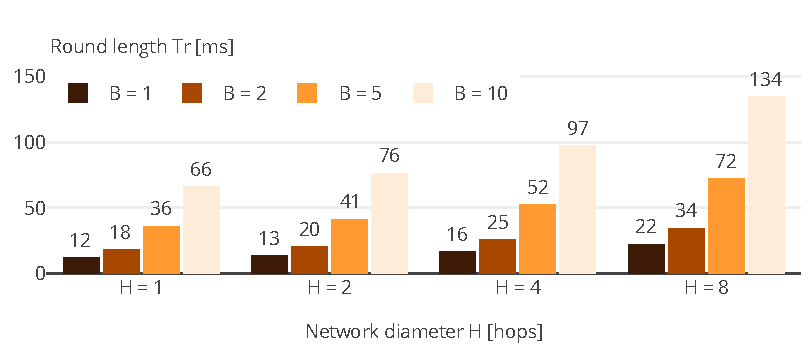
\includegraphics[scale=1]{T=f(H,B)}}
  \end{subfigure}
  \begin{subfigure}{\linewidth}
    \centering
    \href{\ttwfig{Figure-14}}{%
    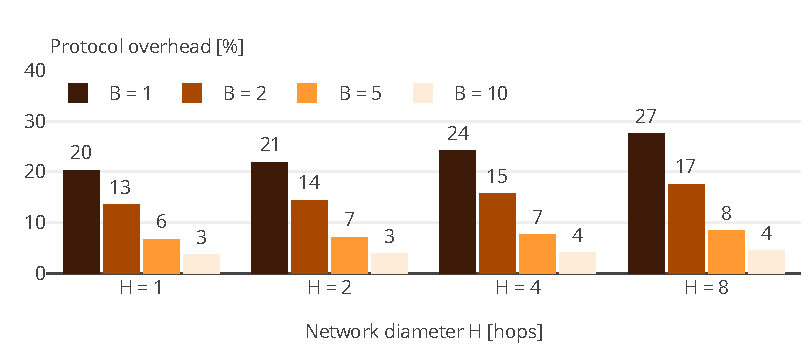
\includegraphics[scale=1]{Overhead=f(H,B)}}
  \end{subfigure}
  \caption{Example values of round length (top) and protocol overhead (bottom) computed using the \TTnet model~(\cref{subsec:model}).
  The protocol overhead is computed as the percentage of time spent to send the beacons relative to the overall communication time for a round containing \nslots slots.
  Payload is set to 16\bytes and we use $N = $2 transmissions in the Glossy floods~\cite{ferrari2011Glossy}.}
  \label{fig:TTWmodel}
\end{figure}
}


The complete \TTnet model is available in Appendix~(\cref{appendix:ttw_artifacts}). We use this model to compute the round length \Tround and the energy savings $E$ for different values of number of slots per rounds (\nslots), message payload size ($L$), network diameter $H$, and number of transmissions in Glossy floods ($N$).
Selected results are shown in \cref{fig:TTWmodel,fig:energy_ratio}.
\linebreak
For example, with $N$ set to 2, it takes less than 100\ms to complete a 10-slot round sending 16-bytes messages over a 4-hop network~(\cref{fig:TTWmodel}, top).



% ------------------------------------------------------------------------------
\subsection{Model Validation}

We now evaluate the runtime execution of our implementation and aim to validate our \TTnet model.
In particular, it is important that the round length model gives safe upper-bounds since the \TTW scheduler relies on the model to schedule messages and tasks: if a round overruns, this may delay the execution of subsequent tasks and cause deadline misses.
We test our \TTnet implementation for different number of slots per round \nslots and payload size $L$, we measure the round length and radio-on time experienced by the different nodes in the network, and we compare the results with the \TTnet model.

\fakepar{Evaluation scenario}
We program the network to execute, one round with \nslots slots, followed by \nslots rounds with one slot.
For each of these rounds, we collect the round length and the radio-on time. Both values are measured in software (\ie the measurement is implemented in the firmware) and use a 32\kHz timer, leading to a measurement accuracy of about 30\us.

\begin{table}
  \centering
  \caption{\triscale parameters for the experimental validation of \TTnet's model}
  \label{table:ttw_triscale_param}
  {\smaller \input{\TablePath/triscale_param.csv}}
\end{table}


\fakepar{Experiment design}
We design the evaluation using the \triscale framework (introduced in \cref{ch:triscale}). The evaluation parameters are listed in \cref{table:ttw_triscale_param}.
Our evaluation scenario is terminating (there is a finite task to accomplish); thus there is no need to test for convergence.
The round length evaluation aims to validate that the \TTnet model is a safe upper-bound; thus, we use the maximum measured round length across all nodes as metric for a run.
For the same reason, we choose a large KPI (95th percentile) and a high confidence level (95\%), which leads to a minimal number of 59 runs per series.
To investigate the reproducibility of the results, we choose the median and a 75\% level of confidence for the variability scores, leading to a minimal number or 3 series.
To evaluate the average savings provided by using communication rounds, we use the median values across nodes as metric.
We perform the evaluation on FlockLab~\cite{FlockLab}, an indoor testbed located in an office building. It has been shown that the experimental conditions on FlockLab exhibits weekly seasonal components~(\cref{subsec:network_profiling}); therefore, to avoid biasing our evaluation, we perform our series of runs using a span of one week, during which we schedule randomly 60 runs per set of parameters. We test our \TTnet implementation using 5, 10, and 30 slots per round, and payloads of 8, 16, and 64\bytes.
The three series of tests were performed between May and October 2019.
The KPI values from our evaluation are listed in~\cref{table:KPIs}.

\afterpage{
\begin{figure}
  \centering
  \href{\ttwfig{Figure-15}}{%
  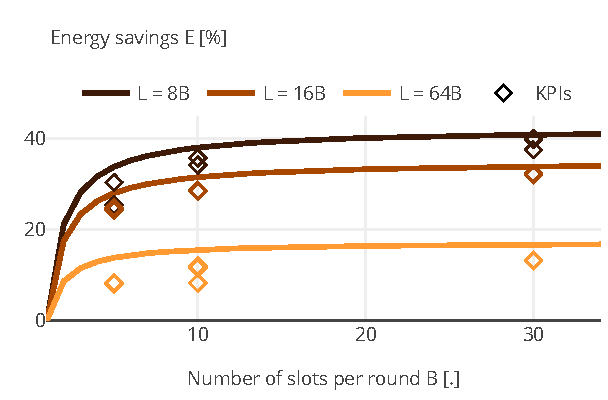
\includegraphics[scale=1]{energy_savings}}
  \caption{Relative radio-on time savings by using rounds compared to single messages.
  \capt{The energy savings induced by a round-based design grow with the number of number of slots per round (X-axis). Conversely, these savings become less significant as the payload size increases (lighter colors).
  The diamonds show our evaluation KPIs and thus estimate, with a probability of 95\%, the average energy savings expected in 95\% of the test runs. $H = 4$, $N = 2$.}}
  \label{fig:energy_ratio}
\end{figure}}

\begin{remark}
  Observe that certain values in~\cref{table:KPIs} are reported with a {\ssymbol{1}} or {\ssymbol{2}} symbol.
  The {\ssymbol{1}} marks series where \triscale independence test fails; this indicates that the metric data do not appear to be \iid and therefore the KPI value loose its predictive power (\ie it does not allow to infer what is the expected performance).
  However, in our evaluation, the autocorrelation plots show no significant differences between the series that passes the test and those that do not~(data available in~\cref{appendix:ttw_artifacts}).
  Moreover, the round length KPI values are almost the same in all series.
  Together, these two facts increase our confidence in the results and suggests that the reported KPIs are robust estimates of the expected performance.\\
  The {\ssymbol{2}} marks series where we could not collect enough data in order to compute the KPIs. This appended in Series 3 due to construction work taking place in the FlockLab building, where many test runs were lost due to sporadic power outages.
  In both cases, the table shows the maximum round length or minimum energy savings metric values obtained across all the runs in the series.
\end{remark}

\fakepar{Results -- Round length}
The results for the round length are extremely stables~(\cref{table:KPIs}):
the differences of KPI values between series are at most one time tick ($\approx$ 30\us), which is our measurement accuracy.
Concretely, this means that, in all series, the largest round length measured by any node is essentially the same.

Furthermore, the KPI values are (i)~very close to and (ii)~consistently lower than the model. By definitions of the KPI, we can estimate with 95\% probability that (at least) 95\% of runs will yield a maximal round length smaller than the KPI value, and thus smaller than the model value.
\cref{fig:exampleSeries} (top) shows the distribution of the round length measurements from all the nodes collected during one series of 60 runs. We observe that the distribution is narrow (less than 300\us of spread), which is expected. Indeed, the \TTnet rounds are fully time-triggered; thus, the measurement differences between nodes mainly come from the difference in execution time of \baloo's end-of-round operations, which is expected to be small.

In our entire evaluation, there was one case where a node reported a value (77.85\ms) larger than the model (77.52\ms). This concerned only one node: in this run%
\footnote{FlockLab test number 66992; data available in~\cref{appendix:ttw_artifacts}.}
the second highest value reported (77.12\ms) was smaller than the model value.
It is hard to know a posteriori what may have cause this.
However, we argue that this one overshoot is more likely imputable to some sporadic hardware delay than due to a miscalibration of the model.

\afterpage{
\begin{figure}
  \centering
  \begin{subfigure}{\linewidth}
    \centering
    \href{\ttwfig{Figure-16}}{%
    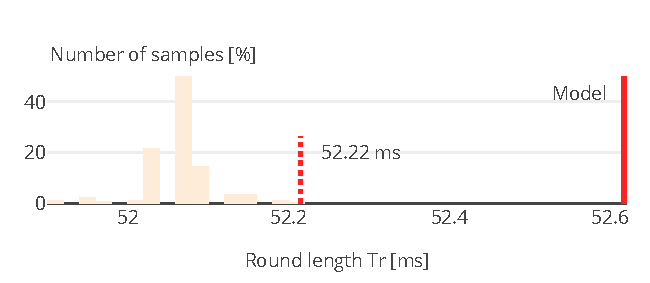
\includegraphics[scale=1]{serie2_T_round_H4_N2_L16_B5}}
  \end{subfigure}
  \begin{subfigure}{\linewidth}
      \centering
      \href{\ttwfig{Figure-16}}{%
      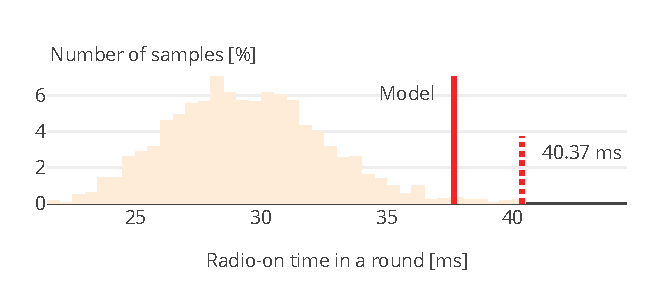
\includegraphics[scale=1]{serie2_T_on_round_H4_N2_L16_B5}}
  \end{subfigure}
  \caption{Distributions of round length (top) and radio-on time (bottom) measurements from all the nodes, collected in one series of 60 runs (Serie 2, $L=16$, $\nslots=5$).
  \capt{
    While the distribution of round length is very narrow, the radio-on time exhibits a much larger spread. We can see that the \TTnet model provides a generally overestimate the radio-on time, which is expected since it assumes that nodes keep their radio on for the entirety of \Tflood~\textup{(}\cref{eq:Ton}\textup{)}, which is not the case in practice: nodes turn the radio off when they have transmitted a packet $N$ times.
  }}
  \label{fig:exampleSeries}
\end{figure}}

\fakepar{Results -- Energy savings}
The energy savings results show more fluctuations than the round length, which is not surprising: (i)~the energy model is less precise and (ii)~the dynamic interference conditions affect the radio-on time, as nodes may need to keep their radio on for a longer share of \Tglossy.
\cref{fig:energy_ratio} shows the model and our energy savings KPIs together.
\cref{fig:exampleSeries} (bottom) shows the distribution of radio-on time measurements from all the nodes, collected in one series of 60 runs: nodes experience significant differences in radio-on time during a round. This is expected since nodes terminate a flood as soon as they have transmitter a packet $N$ times, which happens earlier for nodes that are closer to the initiator,

Overall, the energy savings come from the ``distribution'' of the overhead from sending beacons between the slots. Thus, the more slots (increasing \nslots) and the smaller the slots (decreasing $L$), the more radio-on time is spared by using rounds.
For a payload of 16\bytes, we obtain an average energy savings of about 30\% with only 10 slots per round.

\afterpage{
\begin{landscape}
\begin{table}
  \centering
  \caption{
  KPIs from the performance evaluation described in~\cref{sec:ttw_evaluation_implem} and corresponding model values for the \TTnet round length \Tround and energy savings $E$; other settings: $H=4$ and $N=2$.
  \capt{
    The value marked in bold corresponds to the one case where the round length KPI is larger than the model value.
    {\ssymbol{1}} marks series where \triscale independence test failed.
    {\ssymbol{2}} marks series without enough samples for computing the KPIs.
    In these two cases, reported values are the maximum round length or minimum energy savings metric values for all the runs in the series.
  }}
  \label{table:KPIs}
  {\smaller \input{\TablePath/KPIs.csv}}
\end{table}
\end{landscape}
}

\fakepar{Conclusion}
We validated the tightness and safeness of \TTnet round length model, which was found to be an upper-bound of the effective round length for all but one in about 14k measurements collected.
Furthermore, we showcased that, even with small beacons (2\bytes in our implementation), a round-based design yields significant reduction of radio-on time, and therefore helps minimizing the overall energy consumption~(\feature{Efficiency}).
